\documentclass{article}
\usepackage{graphicx} % Required for inserting images
\usepackage{amsmath, amssymb, mathtools, dirtytalk}

\graphicspath{{Images/}}

\setlength{\oddsidemargin}{0in}
\setlength{\textwidth}{6.5in}
\setlength{\topmargin}{-.55in}
\setlength{\textheight}{9in}
\pagestyle{empty}


\title{Optimization Midterm 1}
\author{Michael Nameika}
\date{March 2023}

\begin{document}

\maketitle
\begin{itemize}
    \item[1.] (22 points) \textbf{Linear Programming}
    Consider the linear program
    \begin{align*}
        \text{minimize} \:\:\:\: &z = -6x_1 - 14x_2 - 13x_3\\
        \text{subject to} \:\:\:\: &x_1 + 4x_2 + 2x_3 \leq 48\\
        &x_1 + 2x_2 + 4x_3 \leq 60\\
        &x_1,x_2,x_3 \geq 0
    \end{align*}
    Answer the related questions.
    \begin{itemize}
        \item[(a)] Put the program in standard form.
        \newline\newline
        Adding the slack variables $s_1, s_2 \geq 0$ to the first and second constraints respectively, we have the program in standard form:
        \begin{align*}
            \text{minimize} \:\:\:\: &z = c^Tx\\
            \text{subject to} \:\:\:\: &Ax = b\\
            &x \geq 0
        \end{align*}
        where 
        \begin{align*}
            A = \begin{pmatrix*}[r]
                1 & 4 & 2 & 1 & 0\\
                1 & 2 & 4 & 0 & 1
            \end{pmatrix*}
            \:\:\:\:\:
            b = \begin{pmatrix*}[r]
                48\\
                60
            \end{pmatrix*}
            \:\:\:\:\:
            c = \begin{pmatrix*}[r]
                -6\\
                -14\\
                -13\\
                0\\
                0
            \end{pmatrix*}
            \:\:\:\:\:
            x = \begin{pmatrix}
                x_1\\
                x_2\\
                x_3\\
                s_1\\
                s_2
            \end{pmatrix}
        \end{align*}        

        \item[(b)] Find the optimal basic feasible solution using the simplex method. After each iteration, show the quantities: $B, y, c_B, \hat{b}, \hat{c}_N, z$. (see Sec. 5.2 for their definitions) Use the origin as your initial guess.
        \newline\newline
        Using MATLAB to solve the linear program (with the initial basis $(s_1,s_2)^T$), we find the following:
        \begin{center}
            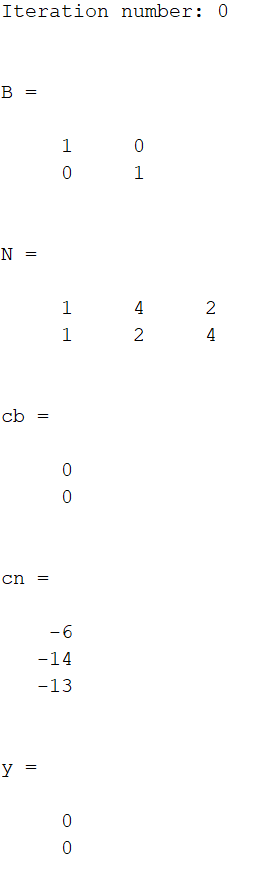
\includegraphics[scale = 0.65]{iteration0Prob1}
            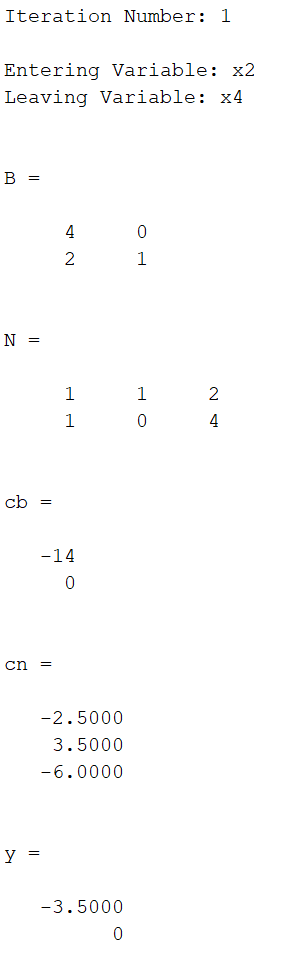
\includegraphics[scale = 0.65]{iteration1Prob1}
            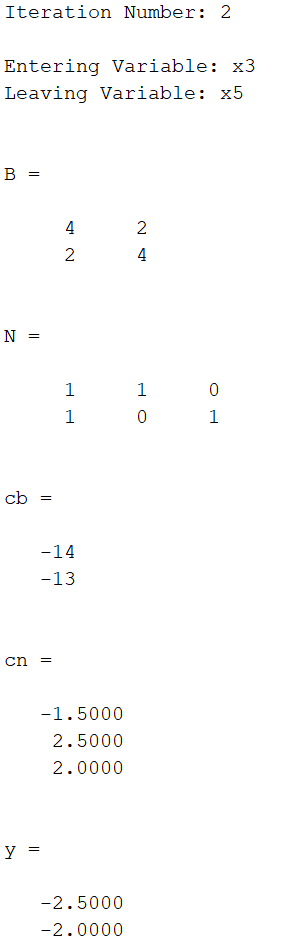
\includegraphics[scale = 0.65]{iteration2Prob1}
            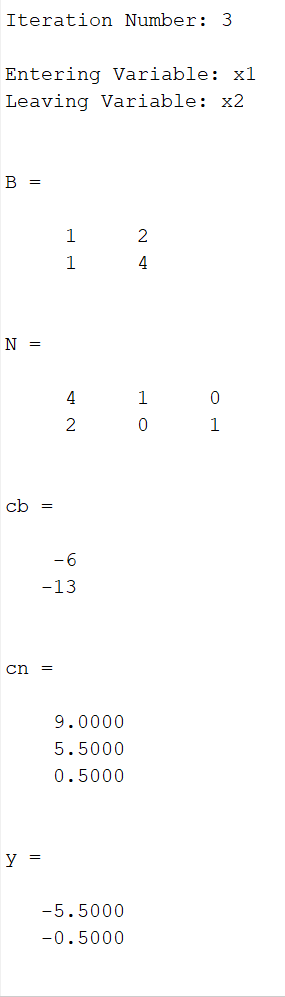
\includegraphics[scale = 0.65]{iteration3Prob1}
        \end{center}
        With an associated minimum value of
        \begin{center}
            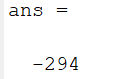
\includegraphics{ansProb1}
        \end{center}
        
        
        
        
        \item[(c)] Find the optimal basic feasible solution using a tableau. Use the origin as your initial guess.
        \newline\newline
        See attached work. Notice that we find the same minimum.
        \newline\newline
    \end{itemize}

    \item[2.] (22 points) \textbf{Least Squares Optimization}
    \newline\newline
    The classic linear least squares problem, often used for data fitting, can be formulated as an unconstrained optimization problem. Given the $m \times 1$ data vector $\mathbf{b}$, the goal is to find the solution or best approximation of the linear system $A\mathbf{x} = \mathbf{b}$, where $A$ is an $m \times n$ real matrix and $\mathbf{x}$ is an $n\times 1$ vector. Answer the following questions associated with the least squares problem.

    \begin{itemize}
        \item[(a)] Define the residual function
        \[r = \|A\mathbf{x} - \mathbf{b}\|_2,\]
        where $\| \cdot \|_2$ denotes the standard two-norm. Show that the residual squared can be formulated as an objective function of an unconstrained optimization problem.
        \newline\newline
        Let $f(\mathbf{x})$ be defined as
        \begin{align*}
            f(\mathbf{x}) &= r^2 = \|A\mathbf{x} - \mathbf{b}\|_2^2 \\
            &= (A\mathbf{x} - \mathbf{b})^T(A\mathbf{x} - \mathbf{b}) \\
            &= (\mathbf{x}^TA^T - \mathbf{b}^T)(A\mathbf{x} - \mathbf{b})\\
            &= \mathbf{x}^TA^TA\mathbf{x} - \mathbf{b}^TA\mathbf{x} - \mathbf{x}^TA^T\mathbf{b} + \mathbf{b}^T\mathbf{b}
        \end{align*}
        Since $\mathbf{x}^TA\mathbf{b}$ is a scalar, we have $(\mathbf{x}^TA\mathbf{b})^T = \mathbf{b}^TA\mathbf{x}$ and so our equation above becomes
        \[f(\mathbf{x}) = \mathbf{x}^TA^TA\mathbf{x} - 2\mathbf{b}^TA\mathbf{x} + \mathbf{b}^T\mathbf{b}\]
        Finally, we have the unconstrained optimization problem is 
        \begin{align*}
            \text{minimize} \:\:\:\:\: &f(\mathbf{x}) = \mathbf{x}^TA^TA\mathbf{x} - 2\mathbf{b}^TA\mathbf{x} + \mathbf{b}^T\mathbf{b}
        \end{align*}
        

        \item[(b)] Find the gradient and Hessian of the objective function in part (a). 
        \newline\newline
        To begin, let $B = A^TA$ and consider the term $\mathbf{x}^TA^TA\mathbf{x} = \mathbf{x}^TB\mathbf{x}$. We wish to find the gradient of this term. Rewriting it as a sum, we have
        \[\mathbf{x}^TB\mathbf{x} = \sum_{i=1}^n\sum_{j = 1}^nb_{ij}x_ix_j\]
        Then the only terms of the above sum that contain $x_i$ are (since $B$ is symmetric):
        \[b_{ii}x_i^2 + 2\sum_{\substack{j=1\\j\neq i}}^nb_{ij}x_jx_i\]
        Differentiating this expression with respect to $x_i$, we have
        \begin{align*}
            \frac{\partial}{\partial x_i} \left(b_{ii}x_i^2 + 2\sum_{\substack{j=1\\j\neq i}}^nb_{ij}x_jx_i\right) &= 2b_{ii}x_i + 2\sum_{\substack{j=1\\j\neq i}}^n b_{ij}x_i
        \end{align*}
        Now let us inspect the $\mathbf{b}^TA\mathbf{x}$. Rewriting as a sum, we have 
        \begin{align*}
            \mathbf{b}^TA\mathbf{x} &= \sum_{j=1}^m\sum_{i=1}^nb_ja_{ji}x_i
        \end{align*}
        Then differentiating with respect to $x_i$, we have
        \begin{align*}
            \frac{\partial}{\partial x_i}\left(\sum_{j=1}^m\sum_{i=1}^nb_ja_{ji}x_i\right) &= \sum_{j=1}^mb_ja_{ji} \\
        \end{align*}
        From this, we can see
        \begin{align*}
            \nabla f(\mathbf{x}) &= 2A^TA\mathbf{x} - 2A^T\mathbf{b}\\
        \end{align*}
        

        \item[(c)] Determine the stationary point, $\mathbf{x}_*$. What is the value of the objective function at the stationary point?
        \newline\newline
        Recall that a stationary point for $f(\mathbf{x})$ occurs when $\nabla f(\mathbf{x}_*) = 0$. Using the equation we found in part (b) for the gradient of $f$ and setting equal to zero, we find
        \begin{align*}
            \nabla f(\mathbf{x}_*) &= 2A^TA\mathbf{x}_* - 2A^T\mathbf{b} = 0\\
            2A^TA\mathbf{x}_* - 2A^T\mathbf{b} &= 0\\
            2A^TA\mathbf{x}_* &= 2A^T\mathbf{b}\\
            A^TA\mathbf{x}_* &= A^T\mathbf{b}
        \end{align*}
        That is, the stationary point $\mathbf{x}_*$ is given by the equation
        \[A^TA\mathbf{x}_* = A^T\mathbf{b}\]
        The value of the function at the point $\mathbf{x}_*$ is
        \begin{align*}
            f(\mathbf{x}_*) &= \mathbf{x}_*^TA^TA\mathbf{x}_* - 2\mathbf{b}^TA\mathbf{x}_* + \mathbf{b}^T\mathbf{b}\\
            &= \mathbf{x}_*^TA^T\mathbf{b} - 2\mathbf{b}^TA\mathbf{x}_* + \mathbf{b}^T\mathbf{b}\\
            &= \mathbf{b}^TA\mathbf{x}_* - 2\mathbf{b}^TA\mathbf{x}_* + \mathbf{b}^T\mathbf{b}\\
            &= \mathbf{b}^T\mathbf{b} - \mathbf{b}^TA\mathbf{x}_*
        \end{align*}

        \item[(d)] What is the stationary point when $A$ is nonsingular? What is the minimizer in this case?
        \newline\newline
        If $A$ is nonsingular, we have that $A^T$ is nonsingular. Then from our work in part (c), we have that
        \begin{align*}
            A^TA\mathbf{x}_* &= A^T\mathbf{b}\\
            (A^T)^{-1}A^TA\mathbf{x}_* &= (A^T)^{-1}A^T\mathbf{b}\\
            A\mathbf{x}_* &= \mathbf{b}\\
            A^{-1}A\mathbf{x}_* &= A^{-1}\mathbf{b} \\
            \mathbf{x}_* &= A^{-1}\mathbf{b}
        \end{align*}
        Using this, we find
        \begin{align*}
            f(\mathbf{x}_*) &= \mathbf{b}^T\mathbf{b} - \mathbf{b}^T\mathbf{b}\\
            &= 0
        \end{align*}

        \item[(e)] Suppose $A^TA$ is positive definite. Prove that the stationary point is a unique minimizer. Hint: consider adding and subtracting the term $\mathbf{x}_*^TA^TA\mathbf{x}_*$.
        \newline\newline
        Proof: Let $A^TA$ be positive definite and $\mathbf{x}_*$ a minimizer of $f(\mathbf{x})$. Suppose by way of contradiction that there exists another minimizer $\mathbf{y}_* \neq \mathbf{x}_*$. Then from our work in part (c), we must have
        \[A^TA\mathbf{y}_* = A^T\mathbf{b}\]
        but since $\mathbf{x}_*$ is also assumed to be a minimizer, we have
        \[A^TA\mathbf{x}_* = A^T\mathbf{b}\]
        That is, we have
        \begin{align*}
            A^TA\mathbf{y}_* &= A^TA\mathbf{x}_* \\
        \end{align*}
        Since $A^TA$ is positive definite, $A^TA$ is nonsingular, by multiplying the above equation on each side by $(A^TA)^{-1}$, we find
        \begin{align*}
            (A^TA)^{-1}A^TA\mathbf{y}_* &= (A^TA)^{-1}A^TA\mathbf{x}_*\\
            \mathbf{y}_* &= \mathbf{x}_*
        \end{align*}
        Contradicting our assumption that $\mathbf{y}_* \neq \mathbf{x}_*$.
        

        \item[(f)] Prescribe a set of conditions on the matrix $A$ to guarantee a unique minimizer. Be as specific as possible. Hint: use your result in part (e).
        \newline\newline
        We require, from part (e), that $A$ be of full rank and that $A^TA$ is positive definite.
        
        
    \end{itemize}

    \item[3.] (22 points) \textbf{Bike Shop}
    \newline\newline
    A small bike shop makes two types of bikes: a basic bike and a deluxe bike. The weekly costs and labor associated with making each bike, as well as the proposed sale price, is summarized in the table below.
    \begin{center}
        \begin{tabular}{||c|c|c|c||}
            \hline
             Type of Bike & Sale Price & Labor & Parts \\
             \hline\hline
             Basic, $x_1$ & \$100 & 2 hours & \$50 \\ 
             \hline
             Deluxe, $x_2$ & \$200 & 3 hours & \$150\\
             \hline
        \end{tabular}
    \end{center}
    Employees can work a maximum of 11 hours per week assembling bikes. The store can spend a maximum of \$500 per week on parts. The store wants to maximize profit. Assume any assembled bike is sold.
    \begin{itemize}
        \item[(a)] Write down a linear program describing this problem. Be sure to include an objective function (weekly income) and all relevant constraints.
        \newline\newline
        A linear program that describes the weekly income is given by
        \begin{align*}
            \text{maximize}\:\:\:\: &z = 100x_1 + 200x_2\\
            \text{subject to} \:\:\: &2x_1 + 3x_2 \leq 11\\
            &50x_1 + 150x_2 \leq 500\\
            &x_1,x_2 \geq 0
        \end{align*}
        

        \item[(b)] Find the optimal basic feasible solution. How many of each type of bike should be made to maximize profit? What is the maximal income? Assuming the labor costs are covered by other funds, is the bike shop making a net profit? Note: Net profit is income minus expenses.
        \newline\newline
        Converting the problem into standard form and running the simplex method code in MATLAB, we find the following optimal basic feasible solution:
        \begin{center}
            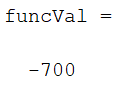
\includegraphics{bikeShopMin}
            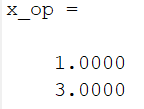
\includegraphics{bikeShopX}
        \end{center}
        That is, the maximimum weekly income is \$700 by building 1 basic bike and 3 deluxe bikes. We are given that the cost of parts for each bike is \$50 for the basic bike and \$150 for the deluxe bike. Using this optimal value, we find that the total cost of parts is \$500. That is, the net profit the shop makes weekly will be \$200, so they are turning a profit.
        \newline\newline


        \item[(c)] The store is considering to allocate more time for bike assembly. The store is also committed to selling both types of bikes. Would adding one more hour on bike assembly (labor) increase profit? What is the new maximal profit? Justify your conclusions with a sensitivity analysis.
        \newline\newline
        Recall that the optimal basis will remain feasible if
        \[B^{-1}(b + \Delta b) \geq 0\]
        Here, we have $B = \begin{pmatrix} 2 & 3\\ 50 & 150 \end{pmatrix}$ and $\Delta b = (1,0)^T$. So 
        \[b + \Delta b = \begin{pmatrix}
            12\\
            500
        \end{pmatrix}\]
        Then
        \[B^{-1}(b + \Delta b) = \begin{pmatrix}
            2\\
            8/3
        \end{pmatrix} \geq 0\]
        So the optimal basis remains feasible. Then the new value of the objective function is
        \begin{align*}
            \bar{z} &= z + y^T\Delta b\\
            &\approx -700 - 33.333\\
            &= -733.333
        \end{align*}
        So the maximal income becomes approximately \$733.33. If we allow $8/3$ of a deluxe bike to be built per week, we find that the total parts cost is still \$500, so the weekly profit increased by approximately 33 dollars after adding one hour to labor.
    \end{itemize}

    \item[4.] (12 points) \textbf{Newton's Method}
    \newline\newline
    The following questions are all related to Newton's method for minimization.
    \begin{itemize}
        \item[(a)] Consider the problem 
        \begin{align*}
            \text{minimize} \:\:\:\:\: &f(\mathbf{x}) = \frac{1}{2}\mathbf{x}^TQ\mathbf{x} - \mathbf{c}^T\mathbf{x},\\
        \end{align*}
        where $Q$ is a positive definite matrix. Prove that Newton's method will determine the minimizer of $f$ in one iteration, regardless of the starting point.
        \newline\newline
        Proof: Let $\mathbf{x}_0$ be some initial guess. Recall that 
        \begin{align*}
            \nabla f(\mathbf{x}) &= Q\mathbf{x} - \mathbf{c}\\
            \nabla^2f(\mathbf{x}) &= Q
        \end{align*}
        Since $Q$ is positive definite, $Q$ is invertible, and so, from Newton's method, we have
        \begin{align*}
            \mathbf{x}_1 &= \mathbf{x}_0 - Q^{-1}(Q\mathbf{x}_0 - \mathbf{c}) \\
            &= \mathbf{x}_0 - Q^{-1}Q\mathbf{x}_0 + Q^{-1}\mathbf{c}\\
            &= \mathbf{x}_0 - \mathbf{x}_0 + Q^{-1}\mathbf{c}\\
            &= Q^{-1}\mathbf{c}
        \end{align*}
        Now, 
        \begin{align*}
            \nabla f(\mathbf{x}_1) &= Q(Q^{-1}\mathbf{c}) - \mathbf{c}\\
            &= \mathbf{c} - \mathbf{c}\\
            &= 0
        \end{align*}
        So $\mathbf{x}_1$ is a stationary point for $f(\mathbf{x})$ and since $Q$ is positive definite, $\nabla^2f(\mathbf{x})$ is positive definite, so $\mathbf{x}_1$ is a minimizer of $f(\mathbf{x})$.
        \newline\newline

        
        \item[(b)] Consider the coefficients
        \[Q = \begin{pmatrix*}[r]
            1 & 2 & 2\\
            2 & 4 & -1\\
            2 & -1 & 4
        \end{pmatrix*},
        \:\:\:\:\:
        \mathbf{c} = \begin{pmatrix}
            1\\
            1\\
            1
        \end{pmatrix}\]
        Is $Q$ positive definite? Apply one exact iteration of Newton's method using initial guess $\mathbf{x}_0 = (0,0,0)^T$. Is this point the minimizer of $f(\mathbf{x})$? Discuss your result in relation to part (a).
        \newline\newline
        Finding the spectra of $Q$, we have
        \[\mathbf{\lambda} = \begin{pmatrix*}[r]
            -1\\
            5\\
            5
        \end{pmatrix*}\]
        So $Q$ is not positive definite since $Q$ has a negative eigenvalue. However, $Q$ is of full rank, so $Q$ is invertible. Then using the initial guess $(0,0,0)^T$ with Newton's method, we find
        \begin{align*}
            \mathbf{x}_1 &= \mathbf{0} - Q^{-1}(Q\mathbf{0} - \mathbf{c})\\
            &= Q^{-1}\mathbf{c}\\
            &= \begin{pmatrix*}[r]
                1/5\\
                1/5\\
                1/5
            \end{pmatrix*}
        \end{align*}
        with an associated value of $f(Q^{-1}\mathbf{c}) = -3/10$.
        \newline
        So the stationary point, similar to part (a), is $\mathbf{x} = Q^{-1}\mathbf{c}$. However, since $Q$ is indefinite, we have that $Q^{-1}\mathbf{c}$ is not the minimizer. We can see this by noticing
        \[f(\mathbf{x}) = -3\]
        for $\mathbf{x} = (-2,1,1)^T$. So $Q^{-1}\mathbf{c}$ is not the minimizer of $f$.
    \end{itemize}
    \item[5.] (22 points) \textbf{More Linear Programming}
    \newline\newline
    Consider the linear program
    \begin{align*}
        \text{maximize} \:\:\:\:\: &z = x_1 + x_2\\
        \text{subject to} \:\:\:\: -&x_1 + x_2 \leq 0\\
        &x_2 \geq 1\\
        &x_1 \leq 3
    \end{align*}
    Answer the related questions.
    \begin{itemize}
        \item[(a)] Sketch the feasible region.
        \newline\newline
        \begin{center}
            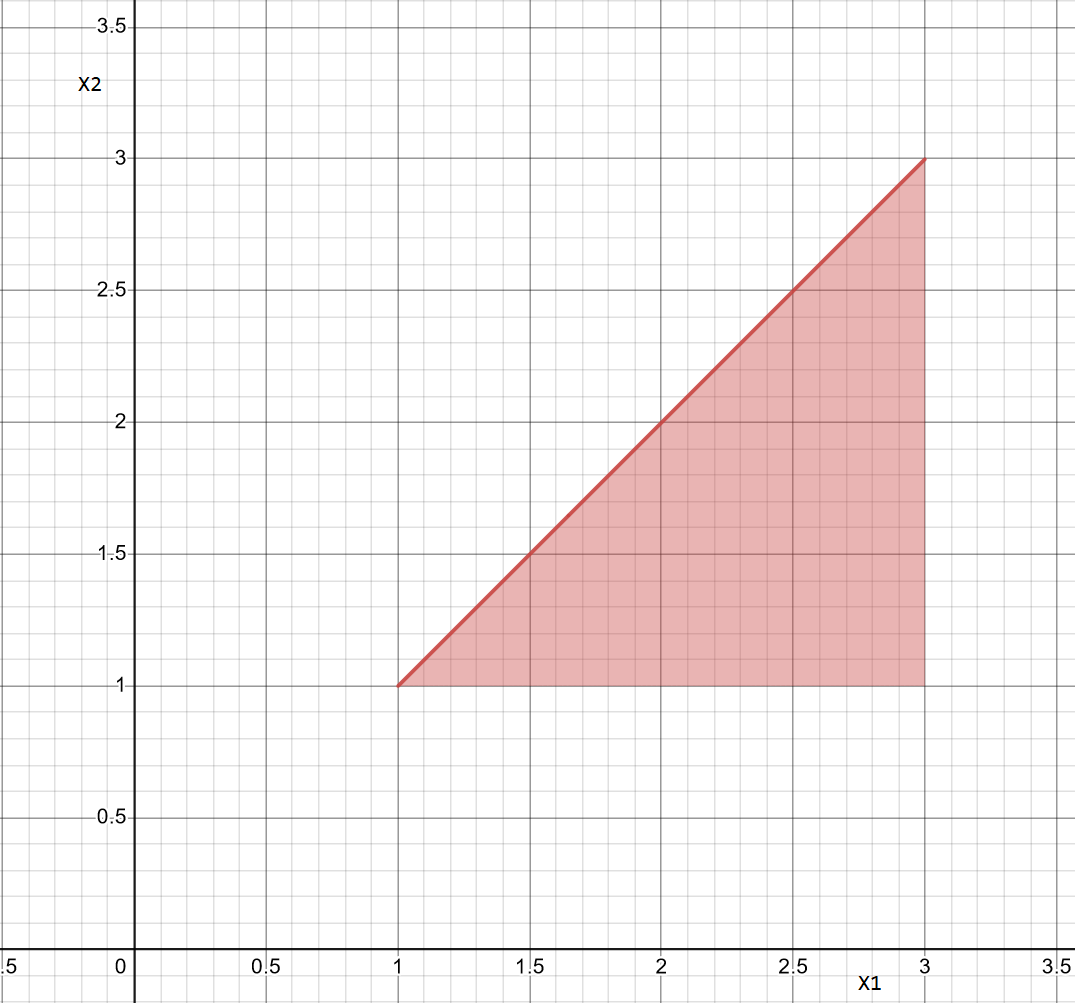
\includegraphics[scale = 0.4]{prob5Feasible_region}
        \end{center}

        \item[(b)] Use the phase-I method to obtain a basic feasible solution.
        \newline\newline
        See attached work.
        \newline

        \item[(c)] Using your result from part (b), solve the linear program.
        \newline\newline
        Using the initial basis we found from the phase-I method, we find the following minimizer for $-z$:
        \begin{center}
            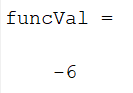
\includegraphics{midtermProb5min}
        \end{center}
        Which corresponds to a maximum value of $z = 6$.
        \newline\newline

        \item[(d)] Write down the dual problem.
        \newline\newline
        To begin, let us change variables to make it clearer to find the dual form. Let $x_1' = 3 - x_1$ and $x_2' = x_2 - 1$. Then our program becomes
        \begin{align*}
            \text{minimize} \:\:\:\:\:\:\:\: &-z = x_1' - x_2' - 4\\
            \text{subject to}\:\:\:\:\:\: &x_1' + x_2' \leq 2\\
            &x_1',x_2' \geq 0
        \end{align*}
        Let $z' = -z + 4$. Our problem then becomes
        \begin{align*}
            \text{minimize} \:\:\:\:\:\:\: &z' = x_1' - x_2'\\
            \text{subject to} \:\:\:\:\:\: &x_1' + x_2' \leq 2\\
            &x_1',x_2' \geq 0
        \end{align*}
        The corresponding dual is then
        \begin{align*}
            \text{maximize} \:\:\:\:\:\: &w' = 2y_1'\\
            \text{subject to} \:\:\:\:\:\: &y_1' \leq 1\\
            &y_1' \leq -1\\
            &y_1' \leq 0
        \end{align*}
        Removing redundant constraints, we have
        \begin{align*}
            \text{maximize} \:\:\:\:\: &w' = 2y_1'\\
            \text{subject to} \:\:\:\:\: &y_1' \leq -1
        \end{align*}
        Let $y_1 = -y_1'$ and convert to a minimization problem:
        \begin{align*}
            \text{minimize} \:\:\:\:\:\:\: &w' = 2y_1\\
            \text{subject to} \:\:\:\:\:\: &y_1 \geq 1
        \end{align*}
        

        \item[(e)] What is the optimal solution of the dual problem? Show that the optimal solution satisfies strong duality.
        \newline\newline
        From part (d), since the dual is one dimensional, we can see that the optimal solution is $w' = 2$, which is also the optimal solution of $z'$. Since $z' = -z + 4$, we have that the optimal solution of $z'$ is the solution to the original problem, just shifted by a scalar factor of $4$. Recall that strong duality states that the optimal solution of the primal problem is also the solution of the dual, which we can see is the case for this problem.
        
    \end{itemize}
\end{itemize}


\end{document}
